\chapter{Обзор существующих реализаций палитр команд}

Впервые палитра команд появилась 1 июля 2011 году в редакторе Sublime Text
2~\cite{sublimetext2changelog}. Вслед за этим подобный функционал был реализован
и в таких программах, как:
Atom\cite{atom},
VSCode\cite{vscode},
JupyterLab\cite{jupyterlab}.

Но это были лишь единичные случаи. В апреле 2017 года появилась альфа версия
приложения Plotinus\cite{plotinus}, которое позволяет добавлять палитру команд в
любое приложение, которое написано с использованием графической библиотеки GTK.

\begin{figure}
	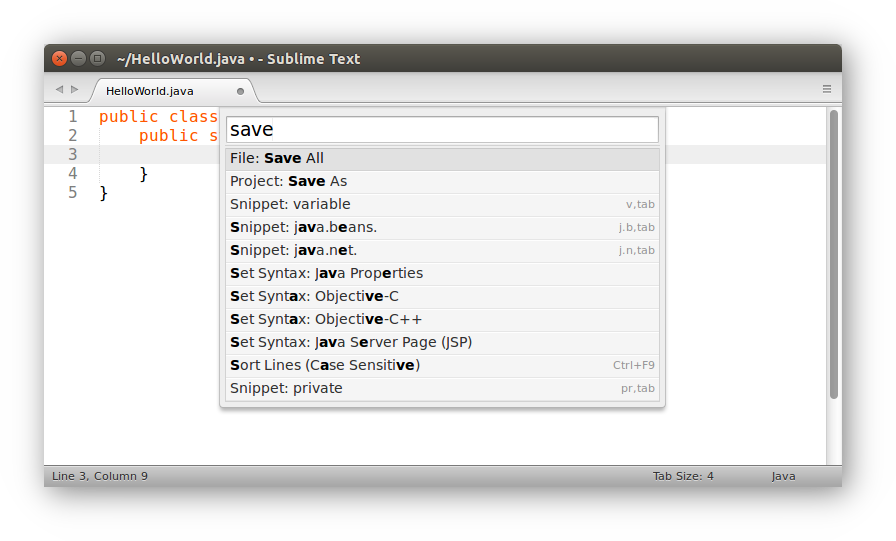
\includegraphics[width=\textwidth]{SublimeText}
	\caption{Sublime Text}
\end{figure}

\begin{figure}
	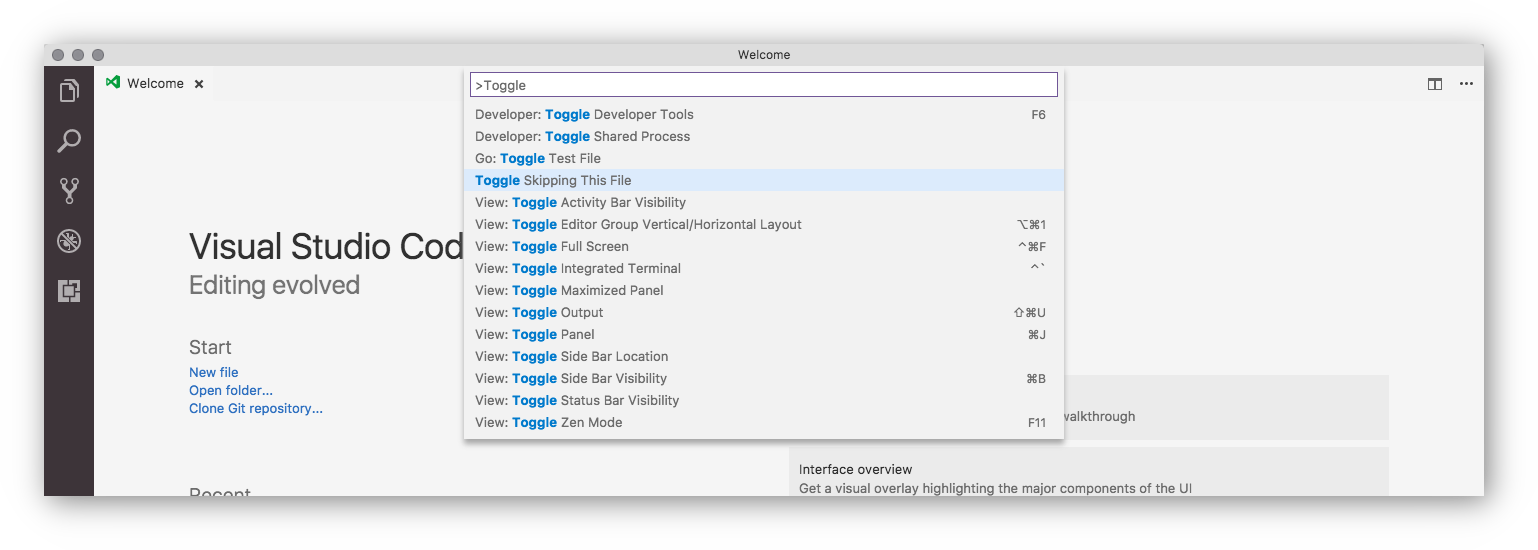
\includegraphics[width=\textwidth]{vscode}
	\caption{VSCode}
\end{figure}

\begin{figure}
	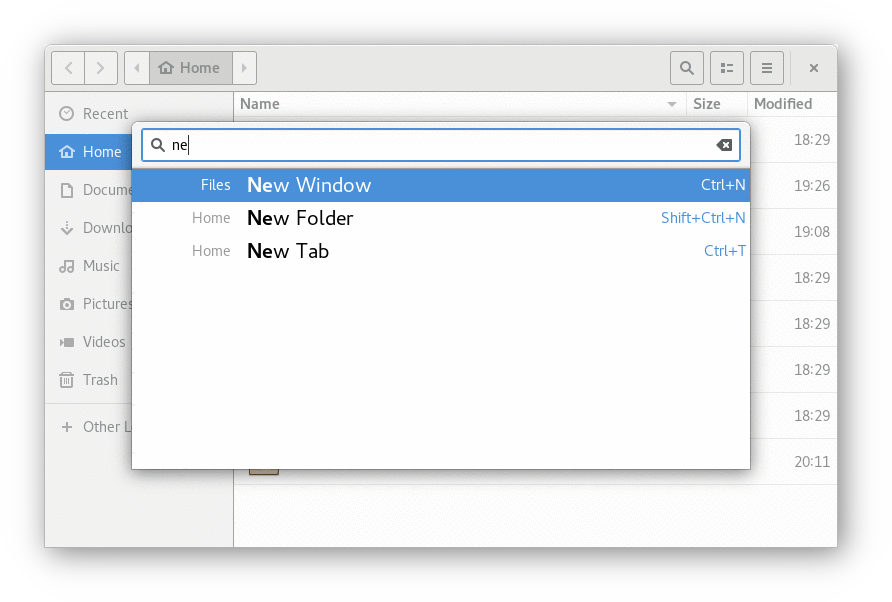
\includegraphics[width=\textwidth]{Plotinus}
	\caption{Plotinus}
\end{figure}

